\documentclass[conference]{IEEEtran}
\IEEEoverridecommandlockouts
% The preceding line is only needed to identify funding in the first footnote. If that is unneeded, please comment it out.
\usepackage{cite}
\usepackage{amsmath,amssymb,amsfonts}
\usepackage{algorithmic}
\usepackage{graphicx}
\usepackage{textcomp}
\def\BibTeX{{\rm B\kern-.05em{\sc i\kern-.025em b}\kern-.08em
    T\kern-.1667em\lower.7ex\hbox{E}\kern-.125emX}}
\begin{document}

\title{Enhancing performance and reliability of Network File System\\
}

\author{
\makebox[.5\linewidth]{ Aswin Babu Karuvally }\\
Department of Computer Applications \\
College of Engineering Trivandrum, KTU\\
Trivandrum, Kerala \\
karuvally@cet.ac.in\\
\and \makebox[.5\linewidth]{ Basith Hameem }\\
Department of Computer Applications \\
College of Engineering Trivandrum, KTU\\
Trivandrum, Kerala \\
basithhameem@cet.ac.in\\
\and \makebox[.5\linewidth]{Ann Jerin Sundar }\\
Department of Computer Applications \\
College of Engineering Trivandrum, KTU\\
Trivandrum, Kerala  \\
annjerinsundar@cet.ac.in\\
\and \makebox[.5\linewidth]{Prof. John Prakash Joseph}\\
Asst. Professor, Department of Computer Applications \\
College of Engineering Trivandrum, KTU\\
Trivandrum, Kerala \\
john@cet.ac.in\\
\\
}
\maketitle

\begin{abstract}
Network File System is a widely used distributed file system that allows the
user to access and manipulate storage on remote computers, as if they were a
part of the local machine. Network File System is notoriously slow in its 
default configuration and if more clients connects to the NFS environment,
it merely accentuates the delay. When configured to deliver faster speeds,
the system suffers from higher risk of data corruption and loss.

This study proposes a number of modifications to the Network File System,
enabling it to provide elevated system performance, while containing
the risk of data loss and corruption. Further, the proposed system behaves
better in congested networks by consuming less bandwidth, ensuring decent
speeds, even during periods of heavy network traffic.
\end{abstract}

\begin{IEEEkeywords}
UNIX,
NFS,
Performance,
Data loss,
Data corruption
\end{IEEEkeywords}

\section{Introduction}
Network File System is a distributed File System protocol primarily used by the  
UNIX family of Operating Systems. It allows users to mount, access and
manipulate disk partitions or directories on a remote computer, as if the
said partition or directory was a part of the local machine. Network File
System was developed as an open standard by SUN Microsystems in 1984\cite{b1}.

NFS is widely used in Local Area Networks to conveniently share data, and
provides users the ability to access their files across the network.
Occasionally, a directory access protocol such as LDAP is combined with NFS,
allowing the users to login to their user accounts from any computer on the 
network.

The main drawback of NFS is the slow read and write speeds it offers with 
the default setup. The current performance enhancing parameters in its 
configuration files, either leave the performance rates unaffected or 
increases the probability of data corruption and loss. Thus the users are 
forced to run the system with the default, slow configuration.

The aforestated configuration diminishes the possibilities of interactive 
computing, and an Operating System requiring access to data on NFS share, 
often ends up freezing the computer, resulting in loss of human productivity.
Moreover, this bottlenecks the computer CPU, wasting valuable computing 
resources. 

This paper proposes a number of changes to the Network File System protocol
which increases the performance of Network File System while reducing
the risk of data corruption and loss. The proposed system also ensures
decent speeds in congested network as it consumes less bandwidth than the 
original NFS implementation and protects the ability of the NFS server to
continue providing access to files during period of peak load.

\section{Background work}
Past studies have proposed new Network File System protocols for
transmitting data over Wide Area Networks. Some other research have dealt
with improving the performance of NFS over wireless links.

A.Muthitacharoen Et al. has proposed a Low Bandwidth Network File System\cite{b2},
which can be used over Wide Area Networks such as the Internet. Though it
minimizes the bandwidth usage of the protocol, it is meant for '90s
era internet. To use it in current scenario would require extensive 
modification to the protocol and it is not compatible with SUN's NFS.

R.Dube Et al. has proposed several changes to the network stack to increase
the performance of NFS over wireless links\cite{b3}. The paper does not suggest
changes to the NFS protocol, instead it tries to optimize the wireless
network stack.

In our literature review, we are yet to come across a research, which
squarely deals with enhancing the performance and reducing data corruption
rates of the widely adopted Network File System protocol, originally
implemented by SUN Microsystems.

\section{Research Methodology}
All the benchmarks for this research study have been done using NFS v4.2.
The NFS environment encompassing the client and server, was emulated using
virtual machines, with the Oracle VirtualBox hypervisor. Virtual Machines 
(VMs) provide a convenient method of simulating target hardware and 
networking infrastructure. The VirtualBox hypervisor was run on RedHat 
Enterprise Linux 7.2, with the hardware being a powerful Xeon workstation
(HP-Z640) to ensure the VMs were not bottlenecked during benchmarks. The VMs
were equipped with an AMD PCnet-FAST III 100 Mbps network adapter which was
bridged to the network, so that each VM represented a real machine on the 
network. Network Address Translation (NAT) was not used as it consumes CPU
resources, which could in turn affect benchmarks. The NFS server and client
VMs were set up to run Debian 9.3 (Stable) as their OS. Debian is a heavily
tested distribution that ships with highly stable packages. Debian was 
chosen so as to minimize the chance of bugs affecting the benchmarks.

The benchmarking tools used include Bonnie ++, Phoronix Test Suite/iozone,
Phoronix Test Suite/dbench, Stand-alone Dbench and the "dd" utility. dd was
used to benchmark NFS performance per client and to cancel out the effects
of client side read/write caches. Dbench is a powerful benchmarking tool
designed to test the performance of NFS and SMB systems. It is capable of
emulating upto 512 clients. All the benchmarks were done with Dbench tool
emulating 6 clients. Higher number of clients not used to avoid choking the
server. Benchmarking was often done through proper combination of all these
tools. When eliminating client side cache effect was required, dd was run
with $conv=fdatasync bs=1K$ options to flush data from cache after write of
each Kilobyte. Each test was run three times, and the average of the results
obtained were taken as the final result.
\section{Working and Typical performance of NFS}
Remote Procedure Call (RPC) in External Data Representation (XDR) format.
RPC allows the NFS client to execute instructions on the server. XDR is a
data representation standard that provides a uniform data format, comprehensible
by a variety of computers. This is one of the factors that provides NFS with
cross platform compatibilty. The working of NFS protocol has been shown in 
Fig. 1.
\begin{figure}[htbp]
\centerline{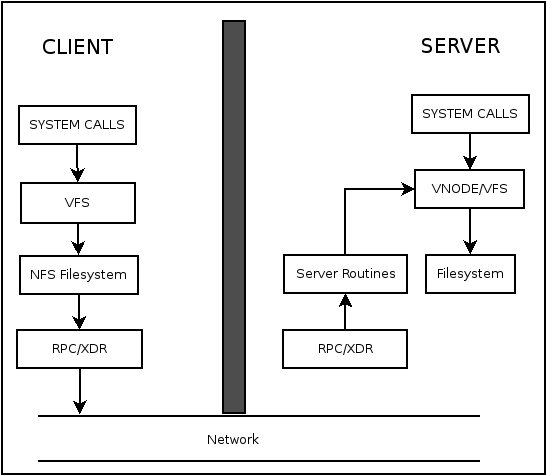
\includegraphics[width=0.5\textwidth,natwidth=400,natheight=300]{Diagram1.png}}
\caption{VFS-NFS handover.}
\label{fig}
\end{figure}
NFS by default runs in what is called server side synchronous mode. In this
mode, when the NFS client receives a write operation, it connects to the
server, requests a write and eventually transfers the data. Once the transfer is
complete, the server syncs the data to its disks. On completion of the sync
operation, the server then returns an acknowledgment message back to the client.
The issue arises with the prolonged waiting period the client endures for the
required acknowledgement. This considerably slows down the system.
Furthermore, clients are often configured to work in client side synchronous
mode, wherein the client is forced to write the data to the server as soon
as it receives the request. This often causes the system to crawl.

The performance of an NFS system with client and server side synchronous
mode turned on was benchmarked with client side options in $/etc/fstab$ set as
\texttt{[rw, sync, hard, intr 0 0]} and the server side options  in $/etc/exports$ set
as \texttt{[rw, no\_root\_squash, subtree\_check]}. The benchmarks were conducted using
dbench utility part of Phoronix Test Suite. This resulted in a performance
of 0.94 MB/s. The speeds obtained are thus clearly sub-optimal. The
peformance graph obtained from the benchmark has been shown in Fig. 2.
\begin{figure}[htbp]
\centerline{\includegraphics[width=0.5\textwidth,natwidth=400,natheight=50]{nfs_working_fig_2.png}}
\caption{Performance with client and server side sync.}
\label{fig}
\end{figure}

\section{Parameters affecting performance}
NFS configuration at the client end are in /etc/fstab file, while at the
server end, the configuration are in /etc/exports file. The commonly used
options are listed in TABLE I and TABLE II
\begin{table}[htbp]
\caption{NFS Options-Client Side}
\begin{center}
\begin{tabular}{|c|c|c|}
\hline
\cline{2-3} 
\textbf{SlNo.} & \textbf{\textit{Option}}& \textbf{\textit{Description}} \\
\hline
1& rw & Read/Write  \\
2& syn & Sync file system with the server  \\
3& hard & NFS requests are retried indefinitely  \\
4& intr & Provided for backward compatibility \\
5& nfsvers & Specifies the nfs versions  \\
6& rsize & Maximum number of bytes when reading data  \\
7& wsize & Maximum number of bytes when writing data  \\
8& udp & Specifies the connection to UDP  \\
9& async & Asynchronous write  \\
\hline
\end{tabular}
\label{tab2}
\end{center}
\end{table}
\begin{table}[htbp]
\caption{NFS Options-Server Side}
\begin{center}
\begin{tabular}{|c|c|c|}
\hline
\cline{2-3} 
\textbf{SlNo.} & \textbf{\textit{Option}}& \textbf{\textit{Description}} \\
\hline
1& rw & Read/Write  \\
2& no-root-squash & Turn off root squashing  \\
3& subtree-check & Specified directory/its subrectory for access  \\
4& async & Synchronous write \\
5& sync & Asynchronous write  \\
\hline
\end{tabular}
\label{tab1}
\end{center}
\end{table}
Various combinations of these options were benchmarked. It was observed 
that most of the options did not improve the performance of the NFS
environment. Server performance remained at 0.94 MB/s.

One significant characteristic observed was that the client side UDP option 
reduced the speeds to 0.77 MB/s. The end of experiments resulted in the 
observation that, only the client and server side asynchronous mode provided
a considerable elevation in performance. 

\section{Performance with Server side ASYNC}
In server side synchronous mode, the server waits till the data has been 
written to its disk before returning the acknowledgment message to the 
client. Server side asynchronous mode changes the behaviour of NFS server 
such that it returns the acknowledgment message as soon as the client 
completes the transfer of data to server's buffer. This has tremendous
impact on the performance of the system.

An NFS system with server side asynchronous mode was benchmarked with the
client side options in $/etc/fstab$ set as\texttt{[rw, sync, hard, intr 0 0]}  and
server side options in $/etc/exports$ set as
\texttt{[rw, no\_root\_squash, no\_subtree\_check, async]}. The test conducted using
dbench resulted in 28.72 MB/s, a huge boost in performance, compared with
side synchronous mode, which returned 0.94 MB/s in dbench. The performance
graph obtained has been shown in Fig 3.
\begin{figure}[htbp]
\centerline{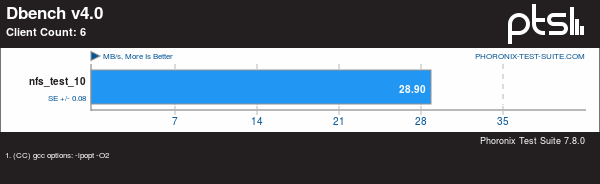
\includegraphics[width=0.5\textwidth,natwidth=400,natheight=300]{server_async_fig.png}}
\caption{Performance with client side sync and server side async.}
\label{fig}
\end{figure}
Benchmarks were also conducted with dd utility, with a block size of 1KB,
file size of 2GB and $fdatasync$ option turned on. The aim was to measure the
worst case performance of server side asynchronous mode. The benchmark
resulted in 7.1 MB/s which was still significantly higher than results
recorded with server side synchronous mode with caching.

The higher performance comes from the fact that the clients no longer have
to wait till the server syncs the data with its disks. Clients can transfer
data to the server's buffer and get on with other tasks such as writing
additiona files. This also means that more number of clients can access the
server in unit time. Still, with the current protocol, it is not advisable
to leave server side async turned on due to the possibility of data loss and
corruption.
\subsection{Reliability concerns with Server side ASYNC}\label{AA}
An advantage of enabling server side asynchronous mode is that, more
clients can access the server in unit time. A side effect is that it can
cause a write queue to form on the client side. A file write can get delayed
and writing a file to the server gives no guarantee that it has been written
to permanent storage. In the event of a server crash, the data written
immediatly before can be lost. Worryingly, the data can be lost from more
than one computer connected to the NFS server.

A client has no means of protecting itself from a server crash. A client has
no NFS cache that is permanent in nature. Even if the client has the lost
file in its primary memory, there is a high chance of loosing it. This is
because, if prior to crash the server was serving a critical file, the
application dependant on the file can crash as well. If the application is
part of the Operating System, it can bring down the whole computer. The
latter is often the case with environments where home directory is served by
an NFS share. Thus, with the current system, server side asynchronous mode
is rather a risky option to leave turned on.

\subsection{Fixing server side ASYNC behaviour}

Once VFS handovers the write request to the NFS client, it transfers the 
received data to the server rather than writing it to the local storage. In
case of data loss, the file cannot be recovered, as the only copy of the
file was in the server's memory. The solution is to create a buffer in the 
client's local storage such that, a copy of all the data written to the
server will be kept with the client.

This buffer is a predefined storage area in the client's secondary memory.
It acts like a ring buffer with a flexible memory size. The oldest files are
deleted once the buffer reaches a predefined size. The NFS client will
maintain a plaintext file in the buffer containing names of each file in the
buffer, its path and hash generated from each file. During an NFS write
operation, the client stores a copy of the file in the buffer area and
updates the metadata file with the information regarding the  new file. The
hash is calculated whenever a file is written to the buffer. To minimize the
CPU overhead for hash calculation, a lightweight hashing algorithm such as
QUARK\cite{b4} or PHOTON\cite{b5} should be used. Fig.4 shows working and structure of the
buffer.
\begin{figure}[htbp]
\centerline{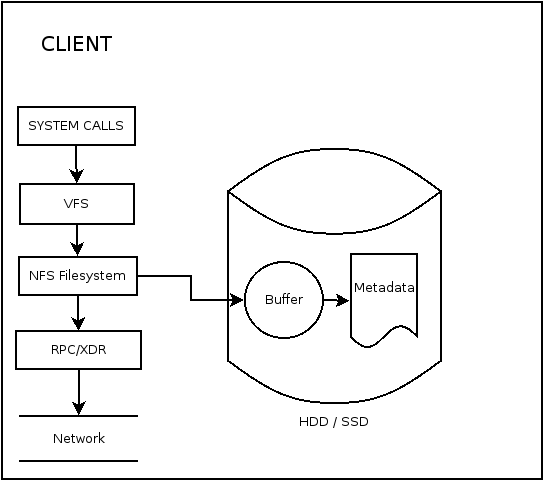
\includegraphics[width=0.5\textwidth,natwidth=400,natheight=50]{fixing_server_async.png}}
\caption{Working and structure of buffer and metadata.}
\label{fig}
\end{figure}
In case of a server crash, the server creates a list of corrupted or lost
files. During the first boot after the crash, the server requests the
metadata file from each client that connects to it. Once the server receives
the metadata, it calculates the hash for the local copy of each file that
is listed in the metadata. If a file is missing or if the hashes do not
match, they are added to the retransmit-list, a list of files to be 
retransmitted from the client. Once the metadata file from a client is fully
scanned, the retransmit list is sent to the client. The client in turn
transmits a new copy of each file in the retransmit list. Fig.5 depicts
the recovery process.
\begin{figure}[htbp]
\centerline{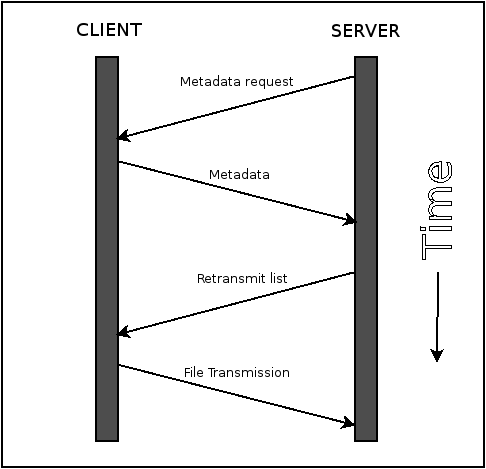
\includegraphics[width=0.5\textwidth,natwidth=400,natheight=50]{error_recovery.png}}
\caption{Error recovery process.}
\label{fig}
\end{figure}




\subsection{Advantages of the proposed solution}
The proposed solution has several advantages, the most important one
being higher security against data corruption and loss. With the current 
system, due to concerns pertaining to data loss, the server side
asynchronous mode is turned off by default. The proposed solution once
implemented, virtually eliminates the chance of data loss and makes it safe
to leave the server side asynchronous mode turned on.

The solution allows the NFS environment to maintain high speeds while
keeping chances of data loss negligibly low. The solution is also easy to
implement as it requires changes to the NFS protocol alone, leaving the
Operating System untouched.

\section{Client side Asynchronous mode}
Client side asynchronous mode is another method, that can be used to improve
the performance of Network File System. Client side asynchronous mode uses
the client's RAM as a giant cache. Once enabled, writes to the NFS server
are written to the client's RAM instead. The file gets written to the server 
only if one of the following conditions are met:
\begin{itemize}
\item Memory fills up
\item An application flushes cache using sync
\item A file is closed with close()
\item A file is locked/unlocked
\item Client shutdown
\end{itemize}

That is, when using client side asynchronous mode, writes to the server are
drastically reduced. This benefits both the client doing the write and the
environment as a whole. For the client, it reduces the number of instances
it has to transfer data to the server. For the server, it reduces the
number of writes it has to deal with in unit time. This also means that the
rest of the clients have to wait less to read/write to the server. dd was
run without arguments and measured 68 MB/s, an increase of 10 MB/s from the
58 MB/s that was measured when dd was run in same configuration with only
server side asynchronous mode turned on.

\subsection{Enhancing client side ASYNC }\label{SCM}
The behaviour of client side asynchronous mode can be further enhanced to 
optimize the performance of an NFS environment. This can be done by
modifying the server such that it keeps two variables, \texttt{max-count} and 
\texttt{current-count}. \texttt{max-count} is the maximum number of clients which can write 
to the NFS server at a time, while \texttt{current-count} is the number of clients 
which are currently writing to the server. \texttt{max-count} is a user configurable
value and can be optimized as per the size of the network.

The client side asynchronous behaviour is modified such that, the clients 
try to write to the server as soon as a threshold is reached. The threshold
is user configurable and can be optimized as per the configuration of the
system. The server initially sets the value of \texttt{current-count}  to 0. The 
server increments the value by one whenever a new client connects. When the
client tries to connect to the server, the server checks if the
\texttt{current-count} is less than \texttt{max-count}. The server allows the client to
connect only if \texttt{max-count - current-count >= 1}. In case the server has
reached its client limit, it denies the connection. The client waits for a
random time \texttt{rand-wait-time} before trying to connect again. \texttt{rand-wait-time} 
is also user configurable and needs to be optimized per the size of the
network. Fig.6 shows the propsed behaviour of client side asynchronous mode
\begin{figure}[htbp]
\centerline{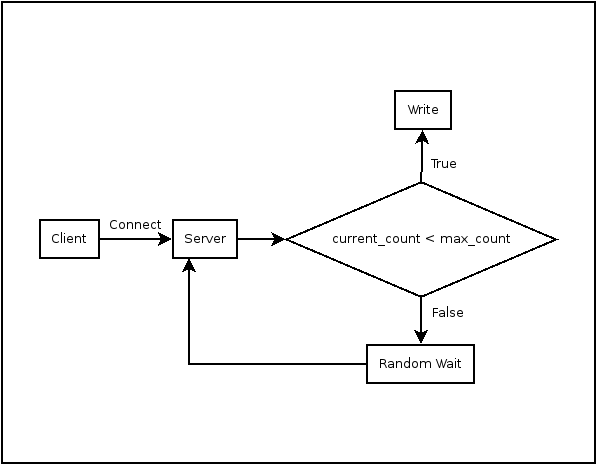
\includegraphics[width=0.5\textwidth,natwidth=400,natheight=100]{enhancing_client_async.png}}
\caption{Proposed client-server behaviour.}
\label{fig}
\end{figure}

\subsection{Advantages of proposed solution}
The proposed solution provides a number of considerable advantages over the
current system. First and foremost, it guards the data against corruption.
With the current system, a particular file can remain in the memory for too
long, while the proposed system forces the NFS client to flush it's caches
when a limit is reached. That is, a file won't remain in the cache for long,
making sure it gets written to the server and to the proposed buffer,
reducing the risk of data corruption.

The current client side asynchronous mode tries to fill up the RAM before
trying to transfer the contents to the buffer. This can negatively affect
the performance of both the applications running on the client and the
network. If a particularly heavy application needs to be loaded, the client 
is forced to flush the caches, thus initiaing the NFS write. The client
will need to wait for the write to complete before the application can be
properly loaded. This introduces unnecessary latency to the system. The 
proposed system also makes sure that the server's capacity is not wasted.
The system makes sure a healthy number of clients get to write to the server
throughout its running time.

Regardless of the number of active clients, the number of clients doing
write to the server will remain a constant. This can improve the overall 
performance of the environment by ensuring that the server can provide 
decent read/write speeds regardless of the state of the environment. Thus
the proposed system can provide a swift and mature NFS behaviour.
\section{Overall performance}
TABLE III summarizes the results of benchmarks obtained during research. The
dd tool in each test was run with options \texttt{bs=1M} and \texttt{count=2048}, meaning
dd created a 2 GB file with block size of 1 MB.
\begin{table}[htbp]
\caption{Benchmark result summary}
\begin{center}
\begin{tabular}{|c|c|c|c|c|}
\hline
\cline{2-3} 
\textbf{SlNo.} & \textbf{\textit{Client}}& \textbf{\textit{Server}}&\textbf{\textit{Dbench(MB/s)}}&\textbf{\textit{dd(MB/s)}} \\
\hline
1& sync & sync & 0.94  &7.3 \\
2& sync & async & 28.72 &58.1 \\
3& async & async & 24.18 & 68.2  \\
4& async & sync & 1.16  & 1.1  \\
\hline
\end{tabular}
\label{tab1}
\end{center}
\end{table}
\section{Conclusion}
Network File System, though introduced in 1984, is still a widely deployed
distributed file system. This study introduces a couple of methods which can
enhance the reliability and performance of the Network File System.

The study proposes a pseudo ring buffer on the client's secondary storage
and proposes changes to the behaviour of NFS client and server to 
drastically reduce the rate of data corruption and loss, when using server
side asynchronous mode. The paper also proposes changes in behaviour of the
NFS client and server when using client side asynchronous mode with an aim 
to reduce data loss and improve overall performance of the system.

Once implemented, the changes suggested in this paper can enhance the
performance of the NFS protocol while bringing down the risks of data
corruption and loss.

\begin{thebibliography}{00}
\bibitem{b1} Russel Sandberg, David Goldberg, Steve Kielman, Den Walsh and Bob Lyon, "Design and Implementation of the Sun Network Filesystem", USENIX Conference and Exhibition, Portland, Oregon, 1985.
\bibitem{b2} Athicha Muthitacharoen, Benjie Chen and David Mazières, "A low-bandwidth network file system" in ACM SIGOPS Operating Systems Review, vol. 35, pp. 174-187, December 2001.
\bibitem{b3} Rohit Dube, Cynthia D. Rais and Satish K. Tripathi, "Improving NFS Performance over Wireless Links" in IEEE Transactions on Computers, vol. 46, pp. 290-298, March 1997.
\bibitem{b4} Jean-Philippe Aumasson, Luca Henzen, Willi Meier, and Marıa Naya-Plasencia, "QUARK: A Lightweight Hash" in Journal of Cryptology, vol. 26, pp. 313-339, April 2013.
\bibitem{b5}Jian Guo, Thomas Peyrin and Axel Poschmann, "The PHOTON Family of Lightweight Hash Functions" in Advances in Cryptology - CRYPTO 2011, 2011.

\end{thebibliography}

\end{document}
